\documentclass{article}
\usepackage{tikz}
\usetikzlibrary{trees}
\begin{document}
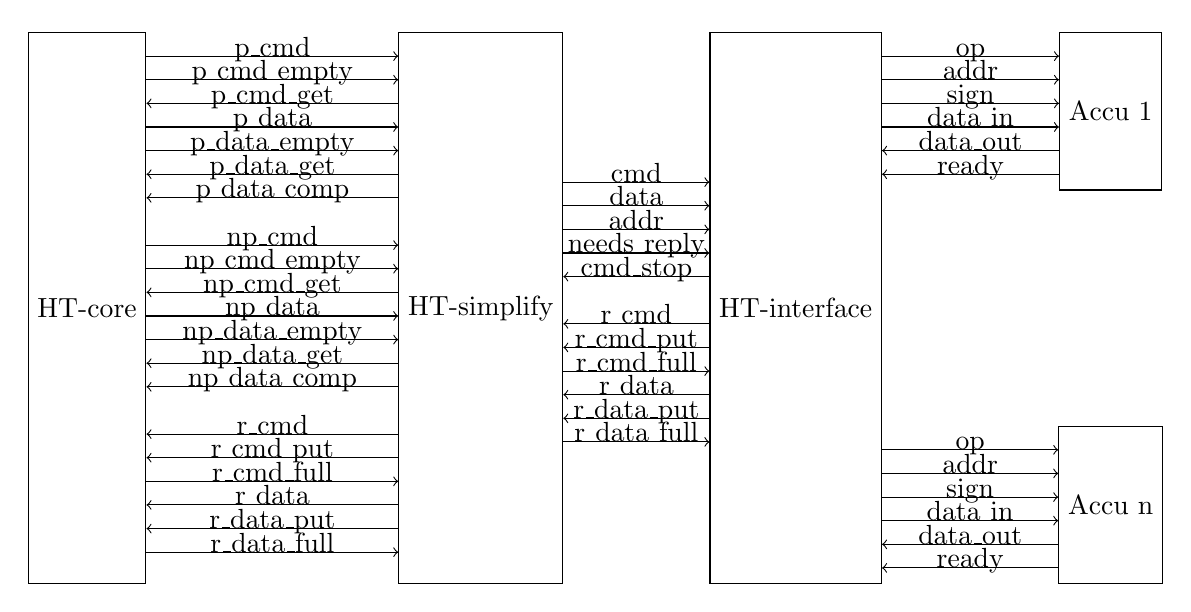
\begin{tikzpicture}
  \tikzstyle{every node}=[rectangle,draw]
  \node[minimum height=7cm] (HT-core)      at (0   ,0) {HT-core};
  \node[minimum height=7cm] (HT-simplify)  at (50mm,0) {HT-simplify};
  \node[minimum height=7cm] (HT-interface) at (90mm,0) {HT-interface};
  \node[minimum height=2cm] (acc1) at (130mm,+25mm) {Accu 1};
  \node[minimum height=2cm] (accn) at (130mm,-25mm) {Accu n};

%% draw connections
  \tikzstyle{every node}=[pos=0.5,draw=none,anchor=base]

%% core <-> simplifier connections
  \newcommand{\mysc}{-3mm}
  \newcommand{\myofs}{32mm}
  \foreach \n/\txt in {  0/p\_cmd,   1/p\_cmd\_empty,   3/p\_data,   4/p\_data\_empty,
                         8/np\_cmd,  9/np\_cmd\_empty, 11/np\_data, 12/np\_data\_empty,
                        18/r\_cmd\_full, 21/r\_data\_full}
    \draw[->] ([yshift=\mysc*\n+\myofs] HT-core.east) -- ([yshift=\mysc*\n+\myofs] HT-simplify.west) node {\txt};
  \foreach \n/\txt in {  2/p\_cmd\_get,   5/p\_data\_get,   6/p\_data\_comp,
                        10/np\_cmd\_get, 13/np\_data\_get, 14/np\_data\_comp,
                        16/r\_cmd,       17/r\_cmd\_put,   19/r\_data,        20/r\_data\_put}
    \draw[<-] ([yshift=\mysc*\n+\myofs] HT-core.east) -- ([yshift=\mysc*\n+\myofs] HT-simplify.west) node {\txt};

%% simplifier <-> mmap interface connections
  \renewcommand{\mysc}{-3mm}
  \renewcommand{\myofs}{16mm}
  \foreach \n/\txt in {  0/cmd, 1/data, 2/addr, 3/needs\_reply,
                         8/r\_cmd\_full, 11/r\_data\_full}
    \draw[->] ([yshift=\mysc*\n+\myofs] HT-simplify.east) -- ([yshift=\mysc*\n+\myofs] HT-interface.west) node {\txt};
  \foreach \n/\txt in {  4/cmd\_stop,
                         6/r\_cmd,        7/r\_cmd\_put,    9/r\_data,        10/r\_data\_put}
    \draw[<-] ([yshift=\mysc*\n+\myofs] HT-simplify.east) -- ([yshift=\mysc*\n+\myofs] HT-interface.west) node {\txt};

%% mmap interface <-> accumulators connections
  \renewcommand{\mysc}{-3mm}
  \renewcommand{\myofs}{7mm}
  \foreach \n/\txt in {  0/op, 1/addr, 2/sign, 3/data\_in} {
    \draw[->] ([yshift= 25mm+\mysc*\n+\myofs] HT-interface.east) -- ([yshift=\mysc*\n+\myofs] acc1.west) node {\txt};
    \draw[->] ([yshift=-25mm+\mysc*\n+\myofs] HT-interface.east) -- ([yshift=\mysc*\n+\myofs] accn.west) node {\txt};
  };
  \foreach \n/\txt in {  4/data\_out, 5/ready} {
    \draw[<-] ([yshift= 25mm+\mysc*\n+\myofs] HT-interface.east) -- ([yshift=\mysc*\n+\myofs] acc1.west) node {\txt};
    \draw[<-] ([yshift=-25mm+\mysc*\n+\myofs] HT-interface.east) -- ([yshift=\mysc*\n+\myofs] accn.west) node {\txt};
  };
\end{tikzpicture}.
\end{document}

